
\chapter{El transistor bipolar de unión}

\section{Introducción}

\subsection{Definición}

El transistor bipolar es un dispositivo semiconducctor multiunión activo. El nombre \textbf{transistor} viene del inglés \textit{transfer resistor}. ``Transfer'' venía a decirnos que se trasmitía una señal desde un electrodo hacia otro, mientras que ``resistor'' nos dice que la señal está modulada por una resistencia que podemos controlar a través de una pequeña corriente. En particular el transistor bipolar de unión (BJT) se utiliza en circuitos para obtener ganancia en corriente/tensión/señal. 

El transistor es un dispositivo semicondcutor con tres regiones dopadas alternativamente. Estas regiones son: \textbf{emisor, base} y \textbf{colector}. Las características de cada una de estas partes están bien definidas: la \textit{base} es una región estrecha en comparación con la longitud de difusión de sus portadores (por la razón que veremos más adelante), y tendrá un dopado diferente al emisor y colector, teniendo dos posibles transistores: tipo PNP y tipo NPN. Finalmente, el emisor tendrá un dopado mayor que el colector, muchas veces representado como P$^+$NP y N$^+$PN. 

Para calcular los voltajes usamos la notación $V_{EB} = V_E - V_B$ siendo $V_E$ la corriente introducida por el emisor. Recordemos que las tres están concectadas a la misma tierra. Así pues tenemos:

\begin{equation*}
    V_{EB} = - V_{BE} = V_E - V_B \qquad 
    V_{CB} = - V_{BC} = V_C - V_B 
\end{equation*}
La configuación más usada es la \textbf{emisor común}, la entrada se aplica entre base y emisor, y la salida se toma entre colector y emisor. Aunque la más intuitiva sea \textbf{base común}. 

\subsection{Regiones de funcionamiento}

Tenemos 4 modos de funcionamiento en función de si el emisor-base está en activa o inversa o si el colector-base está en activa o en inversa. Tenemos pues:

\begin{table}[H] \centering \small
    \begin{tabular}{c|cccc}
        \toprule & Región Activa Inversa & Región Activa Inversa & Región de Corte & Región de Saturación \\ \midrule
        Emisor-Base & Directa $V_{EB}>0$ & Inversa  $V_{EB}<0$ & Inversa  $V_{EB}<0$ & Directa   $V_{EB}>0$\\
        Base-Colector & Inversa $V_{CB}<0$ & Directa  $V_{CB}>0$ & Inversa  $V_{CB}<0$ & Directa  $V_{CB}>0$ \\ \bottomrule        
    \end{tabular}
    \label{Tab:04-01}
    \caption{Resumen de regiones de funcionamiento.}
\end{table}
Veamos ahora una por una las características de los modos de funcionamiento:

\begin{itemize}
    \item La \textbf{zona activa directa} con EB en directa y BC en inversa, es la más usada, ya que es la que genera mayor ganancia de señal y menor distorsión.
    \item La \textbf{región de saturación} con EB en directa y BC en directa, es usada para circuitos lógicos, junto con la región de inversión, ya que como veremos la intensidad que pasa por E$\to$B y B$\to$E es muy parecida, no hay ganancia. 
    \item La \textbf{región de inversión} con EB en inversa y BC también, es usada para circuitos lógicos, junto con la región de saturación, ya que prácticamente no pasa corriente en esta región. Actúan como conmutadores.
    \item La \textbf{región activa inversa} la unión EB está polarizada en inversa y la unión BC lo está en directa. Se podría pensar que el caso activo inverso es aquel en el que el colector funciona como emisor y el emisor como colector, y es cierto, pero al tener un dopado P$^+$NP esto es mucho menos efectivo que activa directa, y no hay ganancia. El uso más común de esta zona de funcionamiento es en circuitos de lógica digital, en los que la ganancia de señal no es un objetivo.  
\end{itemize}

\subsection{Amplfiicación}

El hecho de que el transistor tenga tres terminales va a determinar que tengamos tres configuracioens distintas para su utilización en un circuito, según el terminal que sea común a la entrada y la salida. Se designan por la terminal que es común a los circuitos: 

\begin{table}[H] \centering
    \begin{tabular}{c|ccc}
        \toprule &  Base común & Emisor común & Colector común \\ \midrule
        Entrada  & $I_E$ y $V_{EB}$ & $I_B$ y $V_{EB}$ & $I_B$ y $V_{CB}$  \\
        Salida &  $I_C$ y $V_{CB}$ & $I_C,$ y $V_{EC}$ & $I_E$ y $V_{EC}$\\ \bottomrule        
    \end{tabular}
    \caption{Resumen de señal de entrada y salida.}
    \label{Tab:04-02}
\end{table}
La ganancia de corriente se define como un parámetro que nos dice si y cuánto se ha ampliado la corriente: 

\begin{itemize}
    \item Cuando la base es común no hay ganancia de corriente $I_C/I_E=1$, funciona como fuente de corriente. 
    \item Cuando el emisor es común hay ganancia de corriente $I_C/I_B\gg 1$. 
    \item Cuando el colector es común hay ganancia de corriente $I_E/I_C\gg 1$. 
\end{itemize}
En estos dos últimos casos para un P$^+$NP, una pequeña corriente en la base de entrada, que es muy usada en recombinación, desencadena que a la salida haya corrientes de huecos muy elevadas $I_E$ o $I_C$, que se usan para amplificar la entrada. 

\section{Transistor bipolar ideal}

\subsection{Definición}

El \textbf{transistor bipolar ideal} es aquel transistor en el cual no sucede recombinación/generación ni en las regiones de vaciamiento EB y BC ni en la región Base. Además, consdieraremos que estamos en bajo nivel de inyección (BNI, $n_p, p_n \ll p_p,n_n$), que no hay campo eléctrico en las regiones masivas y el flujo es en una dimensión. Consideramos pues:

\begin{itemize}
    \item Dispositivo con estructura unidimensional.
    \item La región de la base tiene muy poco espesor $W\ll L$.
    \item Corrientes de recombinación-generación en las regiones de vaciamiento despreciables.
    \item Dopado uniforme en las tres zonas del transistor.
    \item Aplicamos la condicción de bajo nivel de inyección. 
\end{itemize}
Nuestro transistor BJT: 

\begin{minipage}{0.45\linewidth} \centering
    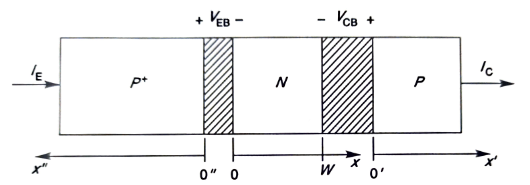
\includegraphics[width=0.6\linewidth]{Cuerpo/Ch_04/Fig-01.png}
\end{minipage} \hfill
\begin{minipage}{0.45\linewidth} \centering
    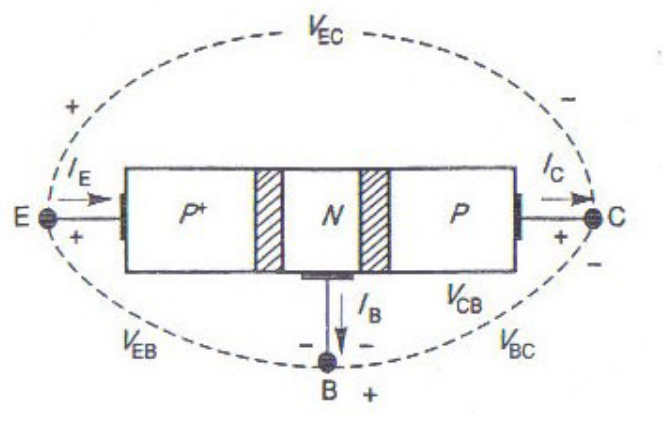
\includegraphics[width=0.6\linewidth]{Cuerpo/Ch_04/Fig-02.png}
\end{minipage}

\subsection{Corrientes}

Para calcular las corrientes usamos los mismos conceptos que en el diodo PN, al menos en el cálculo de las corrientes del emisor y del colector:

\begin{itemize}
    \item La \textbf{corriente del emisor} será la suma de las corrientes debidas a los portadores minoritarios y mayoritarios, tal que:
    
    \begin{equation}
       \text{Tipo P:} \quad I_E = I_{Ep}(0) + I_{En} (0'') \tquad 
       \text{Tipo N:} \quad I_E = I_{En}(0) + I_{Ep} (0'')
    \end{equation}

    \item La \textbf{corriente del colector} será la suma de las corrientes debidas a los portadores minoritarios y mayoritarios, tal que
    
    \begin{equation}
        \text{Tipo P:} \quad I_E = I_{Cp}(W) + I_{En} (0') \tquad 
        \text{Tipo N:} \quad I_E = I_{Cn}(W) + I_{Ep} (0') \tquad 
    \end{equation}

    \item La \textbf{corriente de la base} se calcula  como la suma/diferencia de las dos corrientes, tal que
    
    \begin{equation}
        I_B = I_E - I_C
    \end{equation}
\end{itemize}
Está claro que el problema de las corrientes es mucho más complejo que en la unión PN, principalmente porque ahora tendremos que considerar unas condiciones de contorno más complicadas, ya que pasamos de tener 1 zona de vaciamiento a 2, y además tendremos que considerar la Base. Ahora bien, conceptualmente es igual: primero calculamos las densidades de portadores minoritarios y luego calculamos los valores de las corrientes a través de las ecuaciones que queramos usar. 

La obtención de los resultados de las densidades de portadores minoritarios es un auténtico coñazo, y más con tantas regiones y posibles diferentes materiales, ya que tendremos que considerar 3 longitudes de difusión, 3 coeficientes de difusión... Así pues, em la siguiente imagen resumimos todo el cálculo: 

\begin{figure}[H] \centering
    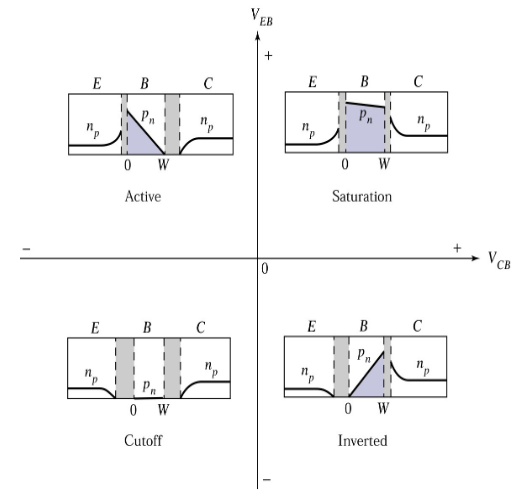
\includegraphics[width=0.6\linewidth]{Cuerpo/Ch_04/Fig-03.png}
\end{figure}

Es importante que en la región de la base $W \ll L$ , ya que esto significa que \textit{los portadores pasan por la base sin sufrir procesos RG}, de lo que se deduce que la ecuación qeu describe correctamente la ecuación es \textit{situación estacionaria, sin iluminiación y sin centros RG} tal que:

\begin{equation*}
    D_P \derivadas{^2 \Delta p_n}{x^2} - \frac{\Delta p_n}{\tau_p} = 0 \longrightarrow \derivadas{^2 \Delta p_n}{x^2} = 0  \longrightarrow \Delta n_p  = A + B \cdot x
\end{equation*}
análogamente en el caso NPN tal que $p_n\to n_p$. Así obtenemos una situación lineal en el interior de la base, mucho más sencilla que la solución exponencial que tendríamos al considerar el caso con RG, con unas ecuaciones de contorno mucho más complicadas. Pese a la ``secillez'' de la ecuación, tenemso que las ecuacioens de las intensidades no son sencillas: 

\begin{equation}
    I_E = I_{Ep} + I_{En} + I_{Ep}' =  q A n_i^2 \ccorchetes{\frac{D_B}{WN_B} + \frac{D_E}{L_EN_E}} \parentesis{e^{qV_{EB}/kT}-1} - q A n_i^2 \frac{D_B}{WN_B} \parentesis{e^{qV_{CB}/kT}-1}
\end{equation}
\begin{equation}
    I_C =  = I_{Cp}' + I_{Cp} + I_{Cn} =  q A n_i^2 {\frac{D_B}{WN_B}} \parentesis{e^{qV_{EB}/kT}-1} - q A n_i^2 \ccorchetes{ \frac{D_B}{WN_B} + \frac{D_C}{L_CN_C} } \parentesis{e^{qV_{CB}/kT}-1}
\end{equation}
\begin{equation}
    I_B = I_E - I_C = I_{B1} + I_{B2} = q A n_i^2 \frac{D_E}{L_EN_E} \parentesis{e^{qV_{EB}/kT}-1} - q A n_i^2\frac{D_C}{L_C N_C} \parentesis{e^{qV_{CB}/kT}-1}
\end{equation}
siendo válidas tanto para PNP como para NPN. Como podemos ver, estas ecuaciones tienen incluidas los valores para activa directa, inversa, corte y saturación. Como podemos ver en la parte superior tenemos 


Resulta muy importante definir los siguientes parámetros:

\begin{itemize}
    \item El \textbf{factor transporte de la base} que mide que nos dice el número de huecos (relativamente) que se lleva el colector frente al emisor:
    \begin{equation}
        \alpha_T = \frac{I_{Cp}}{I_{Ep}}
    \end{equation}
    \item El \textbf{alfa de corriente continua} se define como el factor 
    \begin{equation}
        \alpha_{cc} = \frac{I_C}{I_E}
    \end{equation}
    \item El \textbf{beta de corriente continua} se define como el factor
    \begin{equation}
        \beta_{cc} = \frac{I_C}{I_B}
    \end{equation}
\end{itemize}

\section{Caracterísitcas ideales IV en la zona activa}

Vamos a presentar las variables del circuito necesarias para describir el BJT en activa P$^+$NP. En este caso vamos a tratar la región activa directa, la más intersante por su uso comp amplificador de señal. Estudiemos entonces la corriente de entrada y la corriente de salida de manera separada. Principalmente el concepto de corriente de entrada/señal de entrada depende de que zona del BJT consideremos como ``común'', teniendo tres posiblidades: emisor común (típico), base común y recolector común, tal y como mostramos en la tabla \cref{Tab:04-02}. Veamos que las corrientes, se pueden aproximar ya que 

\begin{equation}
    kT \ll qV_{EB}\Longrightarrow 1 \ll e^{qV_{EB}/kT}\qquad V_{CB} < 0 \Longrightarrow e^{qV_{CB}/kT} \approx 1
\end{equation}

de lo que se deduce: 
\begin{equation}
    I_E \approx q A n_i^2 \ccorchetes{\frac{D_B}{WN_B} + \frac{D_E}{L_EN_E}} e^{qV_{EB}/kT}
\end{equation}
\begin{equation}
    I_C \approx q A n_i^2 {\frac{D_B}{WN_B}} e^{qV_{EB}/kT}
\end{equation}
\begin{equation}
    I_B \approx  A n_i^2 \frac{D_E}{L_EN_E}  e^{qV_{EB}/kT}
\end{equation}


\subsection{Base común}

En la base común tenemos que la entrada es $I_E$ y la salida es $I_C$, y como hemos visto debe ser casi idéntica. Además del alfa de corriente continua y el factor de transporte, nos intersa la  \textbf{eficiencia de inyección de emisor} 

\begin{equation}
    \gamma = \frac{I_{Ep}}{I_E} = \frac{I_{Ep}}{I_{Ep} + I_{En}}
\end{equation}

que basicamente mide el valor de intensidad que es capaz de amplificarse, y es, para nuestras intensidades

\begin{equation*}
    \gamma = \frac{\frac{D_B}{WN_B}}{\frac{D_B}{WN_B}+\frac{D_E}{L_EN_E}}
\end{equation*}
Luego otros valores interesantes son: 

\begin{equation}
    \alpha_{cc} = \frac{I_C}{I_E} = \frac{\frac{D_B}{WN_B}}{\frac{D_B}{WN_B}+\frac{D_E}{L_EN_E}} = \gamma 
\end{equation}
\begin{equation}
    \alpha_T = \frac{I_{Cp}}{I_{Ep}}  = \frac{\frac{D_B}{WN_B}}{\frac{D_B}{WN_B}+\frac{D_E}{L_EN_E}} = \gamma 
\end{equation}

\subsection{Emisor común}

En el emisor común la entrada es $I_B$ y la salida es $I_C$. Veamos que en ese caso tenemos que los voltajes que nos interesan son otros, y por tanto solo tenemos un parámetro de interés, qeu sería la beta de corriente contiunua tal qeu:

\begin{equation*}
    \beta_{cc} = \frac{I_C}{I_B} = \frac{\frac{D_B}{WN_B}}{ \frac{D_E}{L_EN_E}} = \frac{L_E N_E D_B}{D_E W N_B } 
\end{equation*}
la diferencia con la configuración base común es la ganancia que en emisor común es superior. Además sabemos que $W\ll L_E$ y(base estrecha) y que $N_B\ll N_E$ al estar más dopado el emisor que la base. Como podemos por estas dos razones es mucha la ganancia en emisor común frente a la ganancia de base común. 



\section{Desviaciones respecto al transistor ideal}

Hay tres desviaciones respecto al transistor ideal que podemos estudiar: 

\begin{itemize}
    \item Recombinación en la base.
    \item Modulación anchura de base o Efecto Early.
    \item Perforación y avalancha. 
\end{itemize}
Tratemos cada una por separado. 

\subsection{Modulación anchura de la base o Efecto Early}

Básicamente esta desviación nos dice que la anchura real $W$ de la base, cuando cambiamos los voltajes, es diferente, ya que las zonas de vaciamiento cambian junto con $V_{BE}$ y $V_{CB}$, tal que $W (V_{BE}, V_{CB})$. 

\subsection{Perforación y avalancha}

La perforación es la situación física en la cual la modulación de la anchura es tan grande que $W=0$, por lo que las regiones de vaciamiento EB y CB se tocan entre sí. En este punto ya no existe una barrera de potencial que superar por parte de $E_v$ (en el caso de los huecos, PNP), por lo que ahora incrementar el potencial significa aumentar drásticamente el campo eléctrico en el interior lo que lleva una corriente fortísima (corriente de perforación). Cuando aumenta lo suficiente se produce una avalancha. 